%\subsection{Ejercicio 4 - Diana}\label{subsec:ej4}
Para hacer los círculos concéntricos de la diana tan solo hay que ir reduciendo el diámetro de los círculos, sin cambiar las coordenadas. Una página A4 apaisada mide $842x595$, por lo que su centro exacto es ($421$, $297$).

\begin{lstlisting}[language=PostScript, caption=Círculos concéntricos, captionpos=b, label=fun:diana]
% Círculo azul (grande)
newpath 
    0.1 0.1 1 setrgbcolor % Azul
    3 setlinewidth
    421 297 180 0 360 arc   
    fill
stroke

% Círculo rojo
newpath 
    1 0 0 setrgbcolor % Rojo
    3 setlinewidth
    421 297 160 0 360 arc   
    fill
stroke

% Círculo verde
newpath 
    0.33 0.67 0 setrgbcolor % Verde
    3 setlinewidth
    421 297 140 0 360 arc   
    fill
stroke

% Círculo lila
newpath 
    1 0.25 0.7 setrgbcolor % Lila
    3 setlinewidth
    421 297 120 0 360 arc   
    fill
stroke

% Círculo amarillo (pequeño)
newpath 
    1 1 0 setrgbcolor % Amarillo
    3 setlinewidth
    421 297 100 0 360 arc   
    fill
stroke
\end{lstlisting}

Para dibujar la cara uso la imagen creada por el profesor en el ejemplo imagen2.ps(\ref{anexo:imagen2}).\\
\begin{lstlisting}[language=PostScript, caption=Imagen dentro de círculos concéntricos, captionpos=b, label=fun:dianaImagen]
370 250 translate
100 100 scale
14 12  8  [14 0 0 -12 0 12]
{<
eeeeeeeeeeeeeeeeeeeeeeee5577
eeeeeeeeeeeeeeeeeeeeeeee5577
eeffffffffffffffffffffee5577
eeffff0000ffff0000ffffee5577
eeffffffffffffffffffffee5577
eeffffffffffffffffffffee5577
eeffff00ffffffff00ffffee5577
eeffffff00000000ffffffee5577
eeeeeeeeeeeeeeeeeeeeeeee5577
eeeeeeeeeeeeeeeeeeeeeeee5577
5577557755775577557755775577
5577557755775577557755775577
>}
image
\end{lstlisting}

A continuación se muestra la imagen obtenida\myref{fig:4ejer}:
\begin{figure}[H]
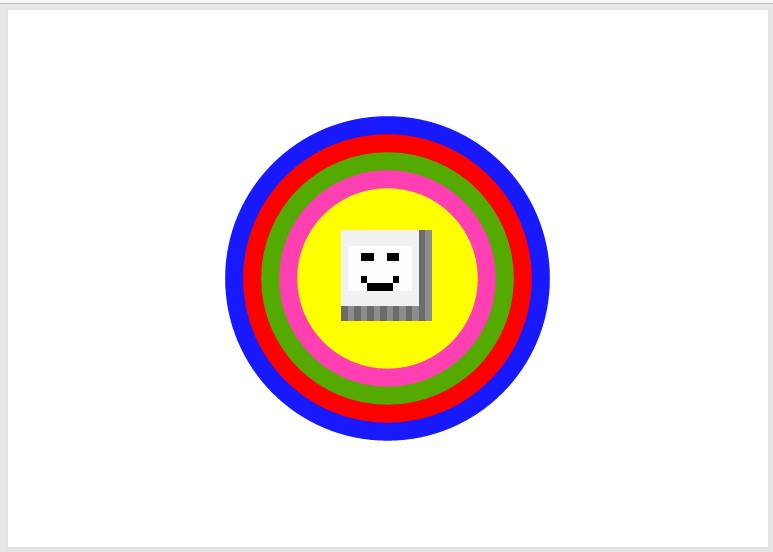
\includegraphics[width=0.9\textwidth]{images/ejer4.jpg}
\caption{Propuesta ejercicio 4.}
\label{fig:4ejer}
\end{figure}

El programa completo se puede ver en el anexo \ref{anexo:ej4}. En el anexo \ref{anexo:pdf4} se puede ver la página pdf generada.